\documentclass[main]{subfiles}

\begin{document}


\chapter{Pruebas sobre el controlador}
\label{chap:test_control}

El objetivo de la presente secci\'on es el de analizar el desempeño del controlador. Nos concentraremos entonces en analizar algunos par\'ametros fundamentales del mismo, es de particular inter\'es conocer la respuesta al escal\'on del sistema para los tres tipos de trayectoria definidos. Modificando la altura del escal\'on se puede determinar la aceleraci\'on m\'axima a la cual podemos someter al sistema en cada trayectoria, esto resulta fundamental a la hora de imponer restricciones sobre la ruta que se desea seguir. Se analizar\'a adem\'as la robustez del controlador implementado, para esto se añade un ruido a los estados realimentados, dicho ruido intenta representar el ruido asociado a las medidas de los sensores. El simulador desarrollado nos permite agregar a cada estado un ruido que cumple con el siguiente modelo:

\begin{equation}
\label{noise}
\eta_i = A_i\cos(\omega t)+\varepsilon(\mu,\sigma)
\end{equation}

Donde $\varepsilon(\mu,\sigma)$ es un ruido gaussiano de media $\mu$ y de desviaci\'on est\'andar $\sigma$.

\section{Respuesta al escal\'on}
Nos centraremos en estudiar las respuestas al escal\'on de los tres tipos de trayectorias. En esta secci\'on no se consideran medidas con ruido, es decir que se conoce el estado a la perfecci\'on.  

\subsection{Trayectoria de hovering}

\subsubsection{Desplazamientos en la direcci\'on vertical}
Se consideran condiciones iniciales nulas. Se fija como setpoint:
\begin{itemize}
\item Prueba 1: ${x_s = 0 m;\quad y_s = 0 m;\quad z_s = 1 m;\quad \theta = 0_s^\circ}$
\item Prueba 2: ${x_s = 0 m;\quad y_s = 0 m;\quad z_s = 100 m;\quad \theta = 0_s^\circ}$
\end{itemize}

No se aprecian variaciones en ninguna de las variables de estado excepto en la posici\'on vertical ($z$) y en la velocidad $v_{q_z}$. Este resultado es perfectamente esperable ya que todas las variables excepto $z$ son iguales al setpoint inicialmente. Para modificar la altura es necesario modificar la velocidad $v_{q_z}$, lo cual explica su variaci\'on. La respuesta al escal\'on para las pruebas uno y dos se muestran en la figura \ref{fig:hov_esc_z}. 
\begin{figure}
  \centering
  \subfloat[Escal\'on de altura 1 m]{\label{fig:Z_1}
  		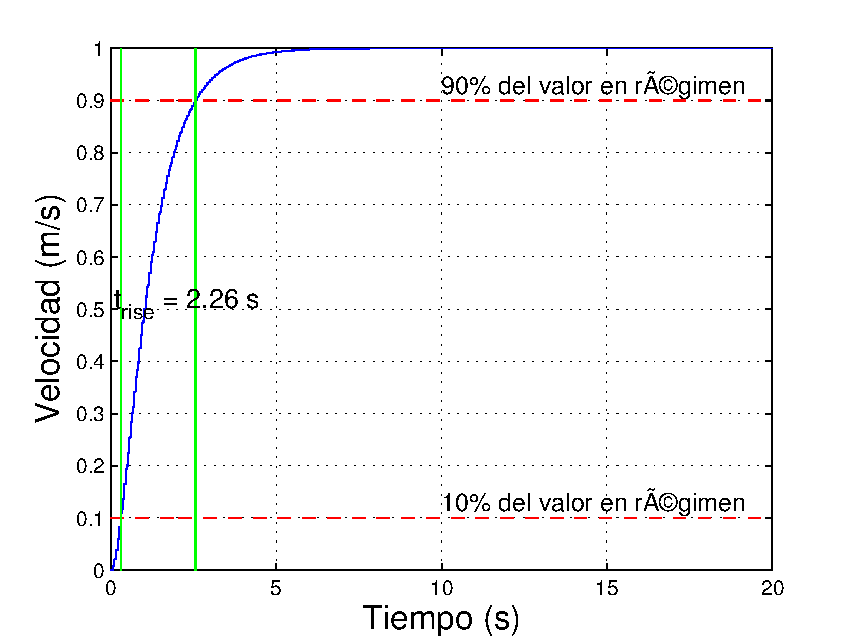
\includegraphics[width=0.5\textwidth]
  			{./pics_test_control/step_hov_z_1.pdf}}
  \subfloat[Escal\'on de altura 100 m]{\label{fig:z_100}
  		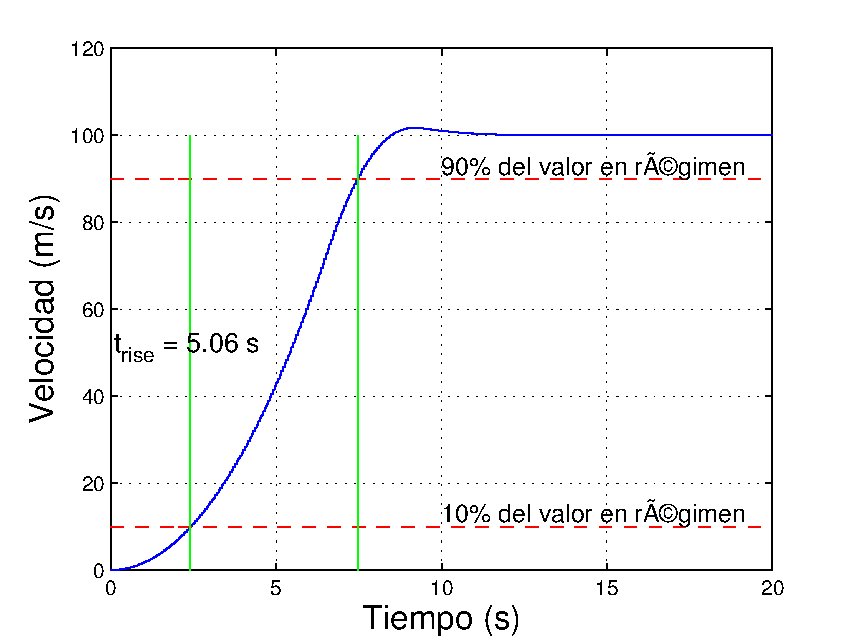
\includegraphics[width=0.5\textwidth]
  			{./pics_test_control/step_hov_z_100.pdf}}
  \caption{Respuesta al escal\'on en la altura}
  \label{fig:hov_esc_z}
\end{figure}

Tanto el tiempo de \emph{rise} como el sobretiro presentado por la respuesta al escal\'on son considerados ampliamente satisfactorios. Para la primera prueba se obtiene un tiempo de \emph{rise} de $2.26 s$ y no hay sobretiro. Para el escal\'on de $100m $ el tiempo de \emph{rise} es de $5.06 s$. En esta prueba aparece un sobretiro inferior a los dos metros. \\

Los resultados obtenidos en la simulaci\'on son ampliamente satisfactorios ya que nos indican que se puede aclanzar un rango de alturas muy amplio en pocos segundos sin que el sistema presente comportamientos que impliquen inestabilidad. Por otra parte se observa en ambas pruebas que una vez alcanzado el valor objetivo se mantiene perfectamente.\\

\begin{figure}
  \centering
  \subfloat[Velocidad en la direcci\'on vertical]{\label{fig:vqz_100}
  		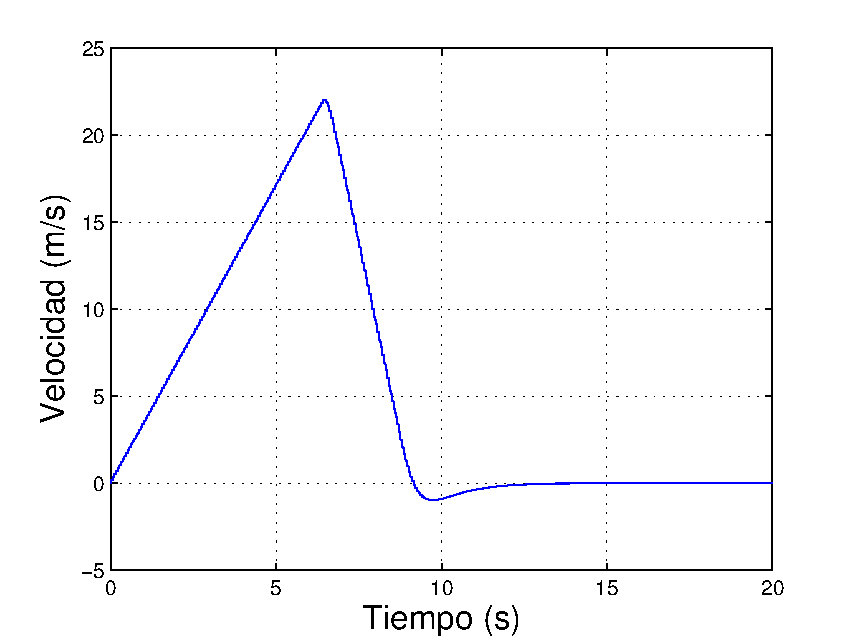
\includegraphics[width=0.5\textwidth]
  			{./pics_test_control/vqz_100.pdf}}
  \subfloat[Velocidad angular del motor 1]{\label{fig:z_100_w}
  		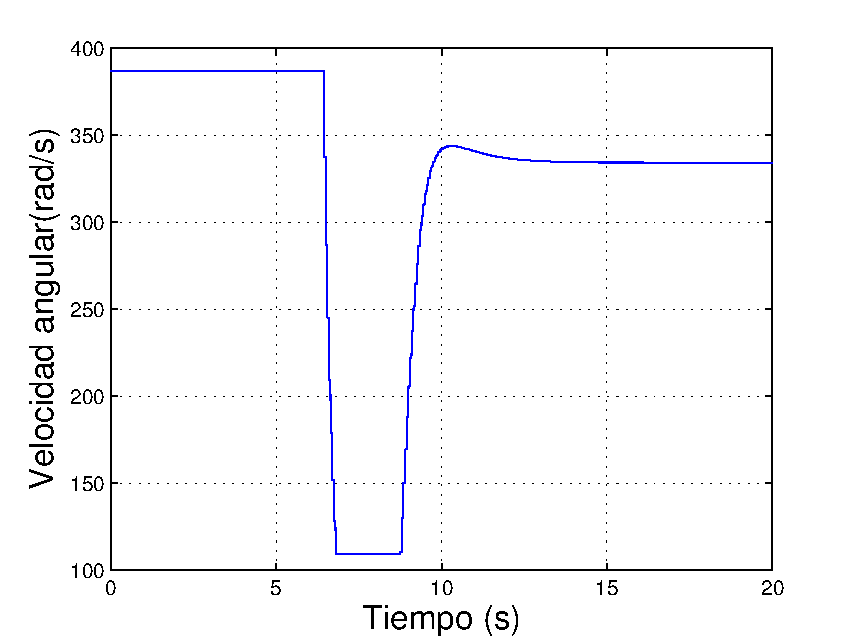
\includegraphics[width=0.5\textwidth]
  			{./pics_test_control/z_100_w.pdf}}
  \caption{Respuestas de la velocidad vertical y la velocidad angular de los motores para el escal\'on de 100m}
  \label{fig:hov_esc_z_otros}
\end{figure}

Si estudiamos la velocidad vertical del sistema en la segunda prueba nos encontramos con que se alcanza la velocidad m\'axima ( $22.05 ms^{-1}$ ) en $6.46 s$. Lo cual implica una aceleraci\'on de $3.41 ms^{-2}$. Por otra parte, luego de alcanzada la velocidad m\'axima esta comienza a disminuir, la aceleraci\'on el tramo en cuesti\'on es de $-7.09ms^{-2}$. Estas aceleraciones son  la m\'axima y m\'inima posible en la direcci\'on vertical ya que, como puede observarse en la figura \ref{fig:z_100_w} la velocidad angular de los motores satura, llegando tanto a su velocidad m\'axima y m\'inima. 

\subsubsection{Desplazamientos en la direcci\'on horizontal}
Partiendo de condiciones iniciales nulas excepto la altura donde se considera $z = 3 m$, se fija el siguiente setpoint:
\begin{itemize}
\item ${x_s = 5 m;\quad y_s = 0 m;\quad z_s = 3 m;\quad \theta = 0_s^\circ}$
\end{itemize}

En la figura \ref{fig:step_x} se observa la trayectoria del sistema solidario al cuadric\'optero a lo largo del tiempo. El comportamiento es acorde a lo esperado. Se observa que el cuadric\'optero tiende a descender inicialmente para luego recuperar su posici\'on inicial. Esto se debe a que en el instante en el cual se produce el escal\'on en el setpoint, se tiene que $z-z_s = 0$, por lo tanto, los t\'erminos de K que dependen de las diferencias no se hacen presentes en la realimentaci\'on, a diferencia de lo que sucede con los t\'erminos que dependen de $x-x_s$.  Todo sucede como si inicialmente el controlador no controlara la altura. En la figura \ref{fig:step_hov_x_z} puede apreciarse que la variaci\'on de la altura es cercana a los $0.3 m$. Se realizaron simulaciones para valores de $x_s > 5 m$, pero los resultados en cuanto a la variaci\'on de las restantes variables de estado no fueron considerados satisfactorios. Por otra parte la aceleraci\'on m\'axima a la cual deber\'ia ser sometido el cuadric\'optero en la direcci\'on horzontal debes ser menor a los $2 ms^{-2}$. Estos \'ultimos aspectos no implican que el control para la condici\'on de hovering sea defectuoso, el controlador fue diseñado linealizando en torno a una trayectoria en la cual $\vec{V} = 0$, por lo tanto es razonable suponer que para no sea adecuado para controlar desplazamientos importantes. En el caso del eje $z$ se obtuvo un desplazamiento importante ya que solamente es necesario modificar la variable $v_{q_z}$ la cual, al tener $\vec{\omega} = 0$ no implica variaciones en ninguna otra variable de estado. Para realizar un desplazamiento seg\'un la direcci\'on horizontal deben modificarse o bien el \'angulo de Roll o bien el \'angulo de Pitch. Sucede que tanto, las velocidades como las posiciones dependen de dichos \'angulos, por lo tanto variaciones importantes en los mismos nos alejan de la condici\'on para la cual se linealiz\'o el sistema.\\

En res\'umen, se desarroll\'o un controlador que nos permite grandes desplazamientos en la direcci\'on vertical $(\approx 100m )$ y desplazamientos inferiores a los $5 m$ en la horizontal, con tiempos de respuesta inferiores a los $5.06 s$ y $2.16 s $ respectivamente, al menos sin presencia de ruido de medici\'on.  

\begin{figure}
  \centering
  \subfloat[Ejes solidarios al cuadric\'optero a lo largo del tiempo]{\label{fig:step_x}
  		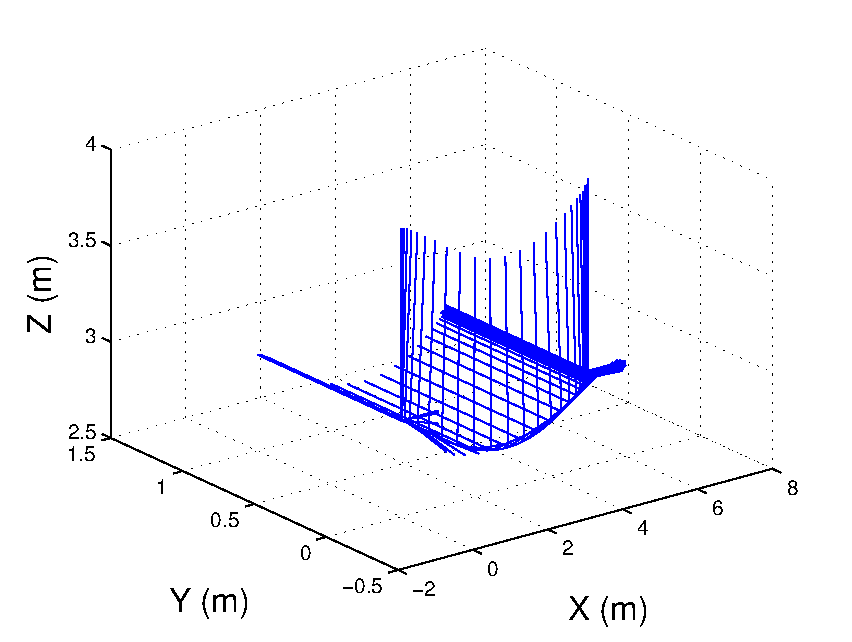
\includegraphics[width=0.35\textwidth]
  			{./pics_test_control/step_x.pdf}}
  \subfloat[Posici\'on seg\'un $\vec{i}_I$]{\label{fig:step_hov_x_5}
  		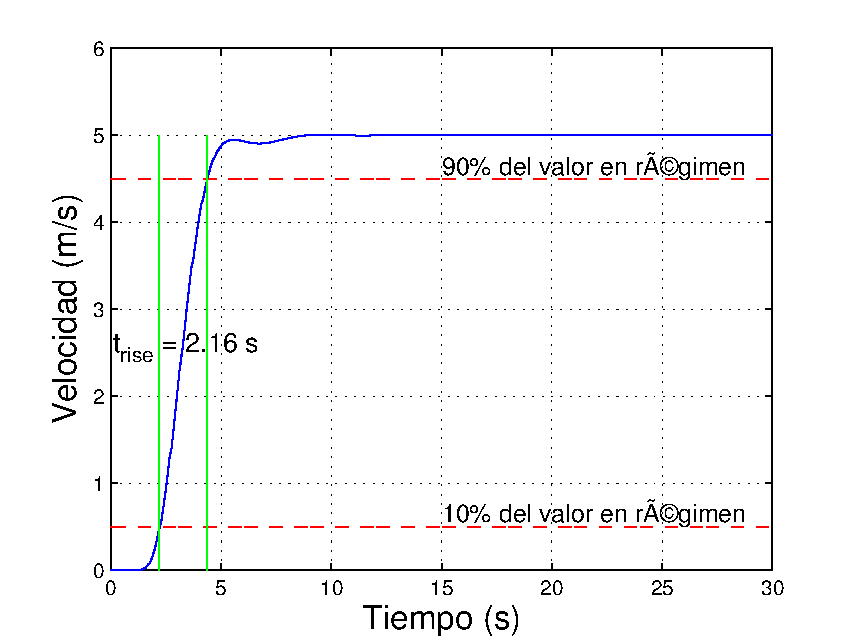
\includegraphics[width=0.35\textwidth]
  			{./pics_test_control/step_hov_x_5.pdf}}
  \subfloat[Altura en m]{\label{fig:step_hov_x_z}
  		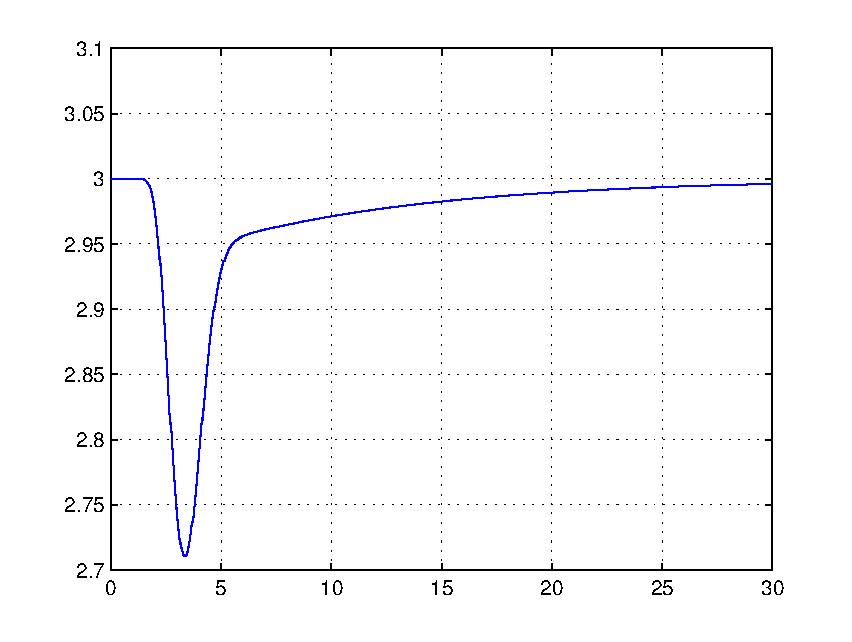
\includegraphics[width=0.35\textwidth]
  			{./pics_test_control/step_hov_x_z.pdf}}
 
  \caption{Escal\'on de 2m en la direcci\'on horizontal}
  \label{fig:hov_esc_x}
\end{figure}


\end{document}